 \section{Sensores}
	Los sensores son dispositivos que permiten a los robots percibir su entorno y obtener información sobre su posición, movimiento, temperatura, proximidad, presión, entre otros aspectos. Estos sensores convierten datos físicos en señales eléctricas que el robot puede procesar para tomar decisiones o realizar tareas.

Se clasifican en:

	\subsection{Sensores Externos}
		\begin{enumerate}
			\item \textbf{Posición}
			\begin{enumerate}
				\item Lineal
				\item Rotativo
			\end{enumerate}
			
			\item \textbf{Velocidad}
			
            Los sensores de velocidad realizan la medición tomando medidas de posición consecutivas a intervalos de tiempo constante, calculando la razón de cambio respecto al tiempo de los valores de posición, o lo determina en forma directa con base en diferentes principios.\cite{saha2010robotics}\\
           
			
			\begin{enumerate}
				\item Todos los sensores de posición:
				Básicamente todos los sensores de posición, cuando se utilizan con ciertos límites de tiempo, pueden dar la velocidad, por ejemplo, el número de pulsos proporcionados por un encóder de posición incremental dividido entre el tiempo consumido en hacerlo. Sin embargo, este método impone una carga computacional sobre el controlador, que podrá estar ocupado por algunas otras operaciones.\\
		
		\begin{figure}[h]
			\centering
			\subfloat[Sensores de posición]{%
				\includegraphics[width=0.4\textwidth]{Velocidadsensoresdeposición.jpg}%
				\label{fig:sensores}
				\cite{Sensordeposición}
			}
			\hfill
		\end{figure}
		
		\begin{figure}[h]
			\centering
			\subfloat[Tacómetro]{%
				\includegraphics[width=0.4\textwidth]{Tacómetro.jpg}%
				\label{fig:Tacómetro}
				\cite{Tacómetro}
			}
			\hfill
		\end{figure}
		
		\begin{figure}[h]
			\centering
			\subfloat[EfectoHall]{%
				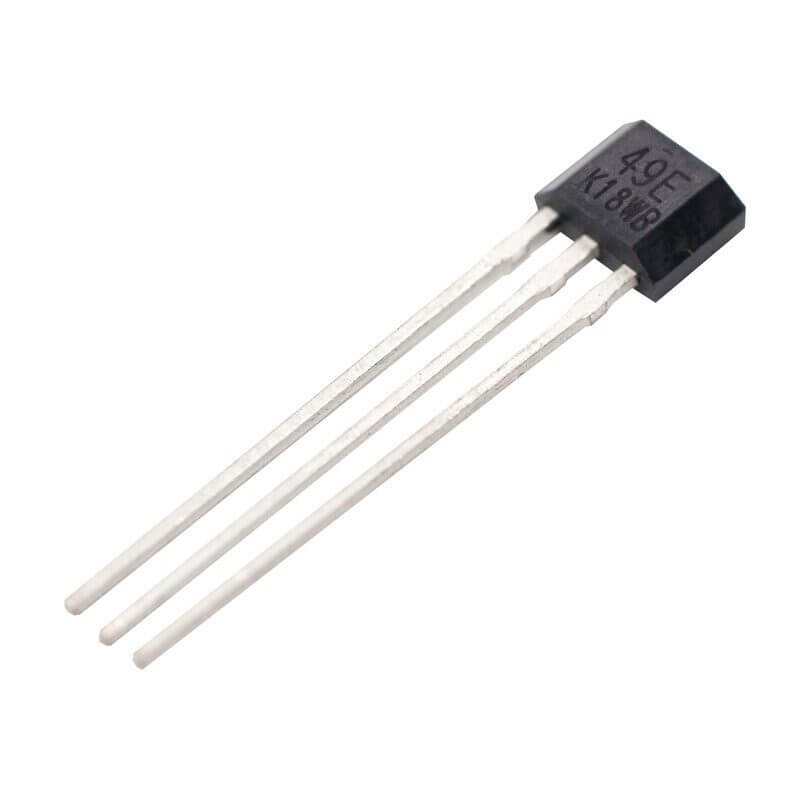
\includegraphics[width=0.4\textwidth]{Hall.jpg}%
				\label{fig:Hall}
				\cite{EfectoHall}
			}
			\hfill
		\end{figure}
				
				\item Tacómetro: Estos sensores pueden encontrar directamente la velocidad en cualquier momento y sin mucha carga computacional. Éstos miden la velocidad de rotación de un elemento. Hay varios tipos de tacómetros en uso, pero un diseño sencillo se basa en la regla de Fleming, que declara que “el voltaje producido es proporcional al índice del acoplamiento inductivo”. Aquí un conductor (básicamente una bobina) se sujeta al elemento rotativo que gira en un campo magnético (estator). Conforme incrementa la velocidad del eje, el voltaje producido en las terminales de las bobinas también aumenta.\cite{saha2010robotics}\\
				
				\item Sensor de efecto Hall: Es un dispositivo que se utiliza para medir la magnitud de un campo magnético. Su función se basa en el fenómeno físico conocido como el efecto Hall, por el cual se genera una diferencia de potencial eléctrico, o voltaje Hall, a través de un material conductor cuando este se encuentra dentro de un campo magnético y se le hace pasar una corriente eléctrica. Este fenómeno fue descubierto en 1879 por el físico estadounidense Edwin Hall.\\
			\end{enumerate}
			
			\item \textbf{Aceleración}
			\begin{enumerate}
				\item Todos los sensores de fuerza
			\end{enumerate}
			
			\item \textbf{Fuerza}
			\begin{enumerate}
				\item Galgas extensométricas
				\item Interruptores de límite
				\item Interruptores piezoeléctricos
			\end{enumerate}
		\end{enumerate}
		
	\subsection{Sensores Internos}
	 \begin{enumerate}
		\item \textbf{Tipo de contacto}
		\begin{enumerate}
			\item Interruptores de límite
			\item Interruptores neumáticos
			\item Sensores piezoeléctricos
			\item Transductores de presión
		\end{enumerate}
		\item \textbf{Tipo sin contacto}
		\begin{enumerate}
			\item Sensores de proximidad
			\item Sensores de efecto Hall
			\item Sensores de microondas
			\item Sensores ultrasónicos
			\item Sensores láser
			\item Sensores de visión
		\end{enumerate}
	\end{enumerate}

Para usar dos imágenes como en \autoref{fig:mascotas}, se utilizó \texttt{subfloat}.
% Dos imágenes de mascotas
\begin{figure}[h]
	\centering
	\subfloat[Perro]{%
		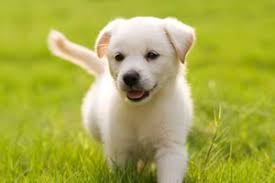
\includegraphics[width=0.4\textwidth]{perro.jpg}%
		\label{fig:perro}
	}
	\hfill
	\subfloat[Gato]{%
		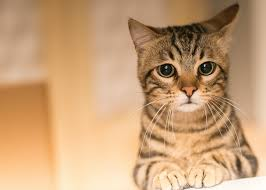
\includegraphics[width=0.4\textwidth]{gato.jpg}%
		\label{fig:gato}
	}
	\caption{Imagen de dos mascotas}
	\label{fig:mascotas}
\end{figure}